% Original author : Leslie Cheng
% Edited by Erik Gabrielsen
% For personal use only
%-------------------------------------

\documentclass[letterpaper,12pt]{article}[leftmargin=*]

\usepackage[empty]{fullpage}
\usepackage{enumitem}
\usepackage{ifxetex}
\ifxetex
  \usepackage{fontspec}
  \usepackage[xetex]{hyperref}
\else
  \usepackage[utf8]{inputenc}
  \usepackage[T1]{fontenc}
  \usepackage[pdftex]{hyperref}
\fi
\usepackage{fontawesome}
\usepackage[sfdefault,light]{FiraSans}
\usepackage{anyfontsize}
\usepackage{xcolor}
\usepackage{tabularx}
\usepackage{graphicx}

%-------------------------------------------------- SETTINGS HERE --------------------------------------------------
% Header settings
\def \fullname {Erik Gabrielsen}
\def \subtitle {}

\def \linkedinicon {\faLinkedin}
\def \linkedinlink {https://linkedin.com/in/dwight-schrute/}
\def \linkedintext {/dwight-schrute}

\def \phoneicon {\faPhone}
\def \phonetext {+47 960 45 058}

\def \emailicon {\faEnvelope}
\def \emaillink {mailto:erik.gabrielsen99@gmail.com}
\def \emailtext {erik.gabrielsen99@gmail.com}

\def \githubicon {\faGithub}
\def \githublink {https://github.com/dwight-schrute}
\def \githubtext {/dwight-schrute}

\def \websiteicon {\faGlobe}
\def \websitelink {https://google.com/}
\def \websitetext {dwightschrute.com}

\def \locationicon {\faMapMarker}
\def \locationtext {Østre Moholt-tun 6, 7050 Trondheim}

\def \birthdayicon {\faBirthdayCake}
\def \birhtdaytext {21.12.1999}

\def \headertype {\headerphoto} % \singlecol or \doublecol

% Misc settings
\def \entryspacing {-0pt}

\def \bulletstyle {\faAngleRight}

% Define colours
\definecolor{primary}{HTML}{000000}
\definecolor{secondary}{HTML}{723976}
\definecolor{accent}{HTML}{263238}
\definecolor{links}{HTML}{1565C0}

%------------------------------------------------------------------------------------------------------------------- 

% Defines to make listing easier
\def \linkedin {\linkedinicon \hspace{3pt}\href{\linkedinlink}{\linkedintext}}
\def \phone {\phoneicon \hspace{3pt}{ \phonetext}}
\def \email {\emailicon \hspace{3pt}\href{\emaillink}{\emailtext}}
\def \github {\githubicon \hspace{3pt}\href{\githublink}{\githubtext}}
\def \website {\websiteicon \hspace{3pt}\href{\websitelink}{\websitetext}}
\def \location {\locationicon \hspace{3pt}{\locationtext} }
\def \birthday {\birthdayicon \hspace{3pt}{\birthdaytext} }

% Adjust margins
\addtolength{\oddsidemargin}{-0.55in}
\addtolength{\evensidemargin}{-0.55in}
\addtolength{\textwidth}{1.1in}
\addtolength{\topmargin}{-0.6in}
\addtolength{\textheight}{1.1in}

% Define the link colours
\hypersetup{
    colorlinks=true,
    urlcolor=links,
}

% Set the margin alignment 
\raggedbottom
\raggedright
\setlength{\tabcolsep}{0in}

%-------------------------
% Custom commands

% Sections
\renewcommand{\section}[2]{\vspace{5pt}
  \colorbox{secondary}{\color{white}\raggedbottom\normalsize\textbf{{#1}{\hspace{7pt}#2}}}
}

% Entry start and end, for spacing
\newcommand{\resumeEntryStart}{\begin{itemize}[leftmargin=2.5mm]}
\newcommand{\resumeEntryEnd}{\end{itemize}\vspace{\entryspacing}}

% Itemized list for the bullet points under an entry, if necessary
\newcommand{\resumeItemListStart}{\begin{itemize}[leftmargin=4.5mm]}
\newcommand{\resumeItemListEnd}{\end{itemize}}

% Resume item
\renewcommand{\labelitemii}{\bulletstyle}
\newcommand{\resumeItem}[1]{
  \item\small{
    {#1 \vspace{-2pt}}
  }
}

% Entry with title, subheading, date(s), and location
\newcommand{\resumeEntryTSDL}[4]{
  \vspace{-1pt}\item[]
    \begin{tabularx}{0.97\textwidth}{X@{\hspace{60pt}}r}
      \textbf{\color{primary}#1} & {\firabook\color{accent}\small#2} \\
      \textit{\color{accent}\small#3} & \textit{\color{accent}\small#4} \\
    \end{tabularx}\vspace{-6pt}
}

% Entry with title and date(s)
\newcommand{\resumeEntryTD}[2]{
  \vspace{-1pt}\item[]
    \begin{tabularx}{0.97\textwidth}{X@{\hspace{60pt}}r}
      \textbf{\color{primary}#1} & {\firabook\color{accent}\small#2} \\
    \end{tabularx}\vspace{-6pt}
}

% Entry for special (skills)
\newcommand{\resumeEntryS}[2]{
  \item[]\small{
    \textbf{\color{primary}#1 }{ #2 \vspace{-6pt}}
  }
}

% Double column header
\newcommand{\doublecol}[6]{
  \begin{tabularx}{\textwidth}{Xr}
    {
      \begin{tabular}[c]{l}
        \fontsize{35}{45}\selectfont{\color{primary}{{\textbf{\fullname}}}} \\
        {\textit{\subtitle}} % You could add a subtitle here
      \end{tabular}
    } & {
      \begin{tabular}[c]{l@{\hspace{1.5em}}l}
        {\small#4} & {\small#1} \\
        {\small#5} & {\small#2} \\
        {\small#6} & {\small#3}
      \end{tabular}
    }
  \end{tabularx}
}

% Single column header
\newcommand{\singlecol}[6]{
  \begin{tabularx}{\textwidth}{Xr}
    {
      \begin{tabular}[b]{l}
        \fontsize{35}{45}\selectfont{\color{primary}{{\textbf{\fullname}}}} \\
        {\textit{\subtitle}} % You could add a subtitle here
      \end{tabular}
    } & {
      \begin{tabular}[c]{l}
        {\small#1} \\
        {\small#2} \\
        {\small#3} \\
        {\small#4} \\
        {\small#5} \\
        {\small#6}
      \end{tabular}
    }
  \end{tabularx}
}

\newcommand{\headerphoto}[6]{
\begin{tabularx}{\textwidth}{Xr}
    {
      \begin{tabular}[b]{l}
        \fontsize{35}{45}\selectfont{\color{primary}{{\textbf{\fullname}}}} \\
        {\small#4 \quad \small#5} \\
        {\small \faBirthdayCake \hspace{3pt}21.12.1999 \quad \small \location}
      \end{tabular}
    } & {
      \begin{tabular}{l}
        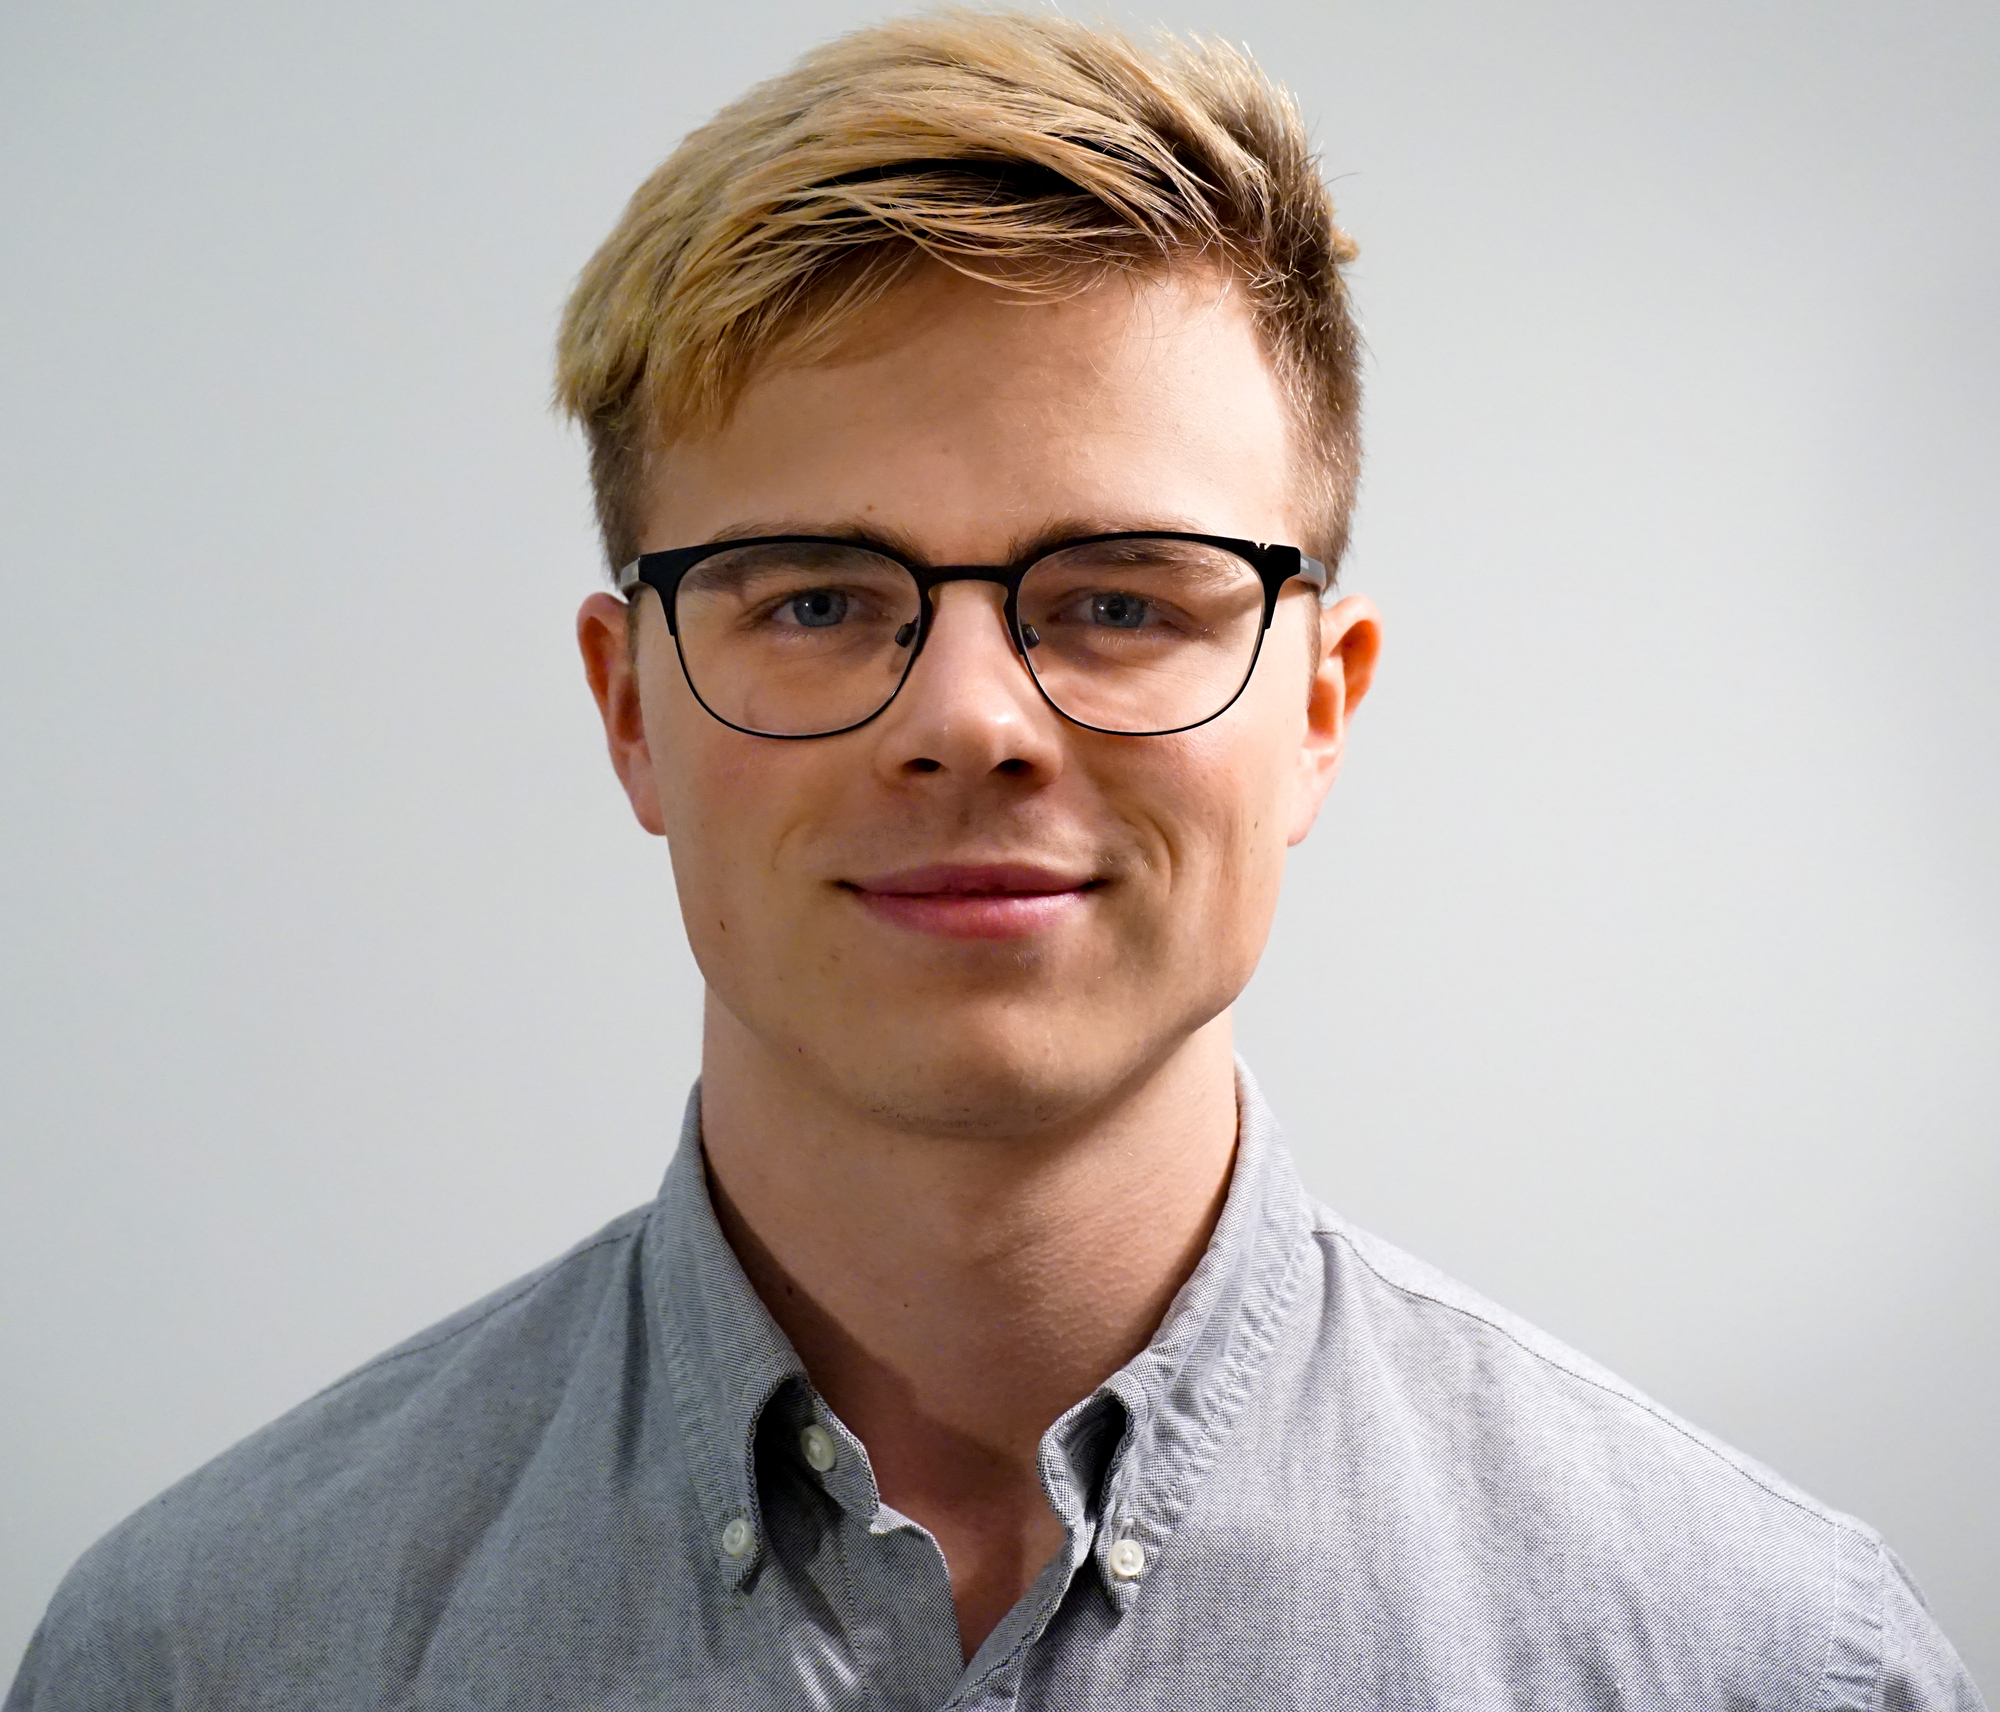
\includegraphics[width = 0.25\textwidth]{profilePic_smaller.jpg}
      \end{tabular}
    }
  \end{tabularx}
}

\begin{document}
%-------------------------------------------------- BEGIN HERE --------------------------------------------------

%---------------------------------------------------- HEADER ----------------------------------------------------

\headertype{\linkedin}{\github}{\website}{\phone}{\email}{} % Set the order of items here
\vspace{-40pt} % Set a negative value to push the body up, and the opposite

%-------------------------------------------------- EDUCATION --------------------------------------------------
\section{\faInfo}{Oppsummering}

\resumeEntryStart
\resumeItemListStart
      \resumeItem {Tredjeårsstudent ved Elektronisk systemdesign og innovasjon på NTNU}
      \resumeItem {Medlem i hardwaregruppa i \href{https://ascendntnu.no/}{Ascend NTNU} }
      \resumeItem{Fem års arbeidserfaring og fagbrev i laboratoriefaget}
      \resumeItem{Utført førstegangstjeneste som radiooperatør i Sjøforsvaret med svært god attest}

    \resumeItemListEnd
\resumeEntryEnd


\section{\faGraduationCap}{Utdanning}

  \resumeEntryStart
    \resumeEntryTSDL
      {Elektronisk Systemdesign og Innovasjon \normalfont(MTELSYS)}{2020 -- Nå}
      {Norges teknisk-naturvitenskapelige universitet}{Trondheim}
    
    \resumeEntryTSDL
    {Sjøforsvarets Radiooperatør Kurs {\normalfont(CIS-1), samt} Røykdykkerkurs}{2019}
    {Tordenskjold}{Bergen}
    
    \resumeEntryTSDL
    {Fagbrev, Laboratoriefaget}{2019}
    {Elkem Technology}{Kristiansand}
    
    \resumeEntryTSDL
    {Tekniske og Allmenne Fag \normalfont(TAF)}{2015 -- 2019}
    {Kvadraturen skolesenter}{Kristiansand}
    
  \resumeEntryEnd

\section{\faSuitcase}{Erfaring}

  \resumeEntryStart
    \resumeEntryTSDL
      {Ascend NTNU}{Sep. 2022 -- Nå}
      {Hardware Medlem}{Trondheim}
    \resumeItemListStart
      \resumeItem {Sentral rolle i utvikling, prototyping og testing av drone til bruk i konkurranse}
      \resumeItem {Hovedansvar for PCB design}
    \resumeItemListEnd
  \resumeEntryEnd

  \resumeEntryStart
    \resumeEntryTSDL
      {Norges teknisk-naturvitenskapelige universitet}{Jun. 2021 -- Aug. 2022}
      {Læringsassistent}{Trondheim}
    \resumeItemListStart
      \resumeItem {Deltidsansatt på IE fakultetet som læringsassistent i faget \textit{Innføring i analog og digital elektronikk}}
      \resumeItem {Videreutvikling av faget sommeren 2021 og 2022}
    \resumeItemListEnd
  \resumeEntryEnd

  \resumeEntryStart
    \resumeEntryTSDL
      {Sjøforsvaret}{Sep. 2019 -- Aug. 2020}
      {Radiooperatør}{KNM Skjold}
    \resumeItemListStart
        \resumeItem {Operasjon, vedlikehold og administrasjon av fartøyets sambandsstasjoner}
        \resumeItem {Forfremmet til Ledende Menig (ULM)}
    \resumeItemListEnd
  \resumeEntryEnd
\newpage
  \resumeEntryStart
    \resumeEntryTSDL
      {Elkem Technology}{Aug. 2015 -- Sep. 2019}
      {Lærling, laboratorieassistent}{Kristiansand}
    \resumeItemListStart
      \resumeItem {Prøvepreparering, homogenisering og kjemisk analyse ved bruk av en rekke kvantitative og kvalitative analysemetoder}
      \resumeItem {Søtte under utarbeidelse av prøvestandarder innenfor ferrosilisium}
      \resumeItem {Bidratt til forskning på karbonbidrag i silisium fra plastposer}
      \resumeItem{Samarbeid med SINTEF i prosjektet \href{https://ree4eu.eu/}{REE4EU} -- gjenvinning av sjeldne jordarter}
    \resumeItemListEnd
  \resumeEntryEnd


%--------------------------------------------------Projects PROJECTS --------------------------------------------------
\section{\faRocket}{Fritid og verv}

  \resumeEntryStart
    \resumeEntryTD
      {Hardwaremedlem, Ascend}{2022 -- Nå}
    \resumeItemListStart
      \resumeItem {Ascend er et studentdrevet teknisk verv som spesialiserer seg på å lage droner til konkurranse}
    \resumeItemListEnd
  \resumeEntryEnd

  \resumeEntryStart
    \resumeEntryTD
      {Nestleder i linjeforeningens HaandbrygerCommitee}{2020 -- 2022}
  \resumeEntryEnd

  \resumeEntryStart
    \resumeEntryTD
      {Diverse hobbyprosjekter}{}
    \resumeItemListStart
      \resumeItem{Urtehage med automatisk vanning}
      \resumeItem{Stoppeklokke til bruk på trening}
      \resumeItem{Ansiktsgjenkjenning på ytterdøren i kollektivet}
    \resumeItemListEnd
  \resumeEntryEnd


\section{\faUsers}{Referanser}
\begin{tabularx}{\textwidth}{XX} {
 \resumeEntryStart
    \resumeEntryTSDL
      {Teisrud, Hege -- \normalfont Sjef}{}
      {Laboratorieingeniør, Elkem Technology}{}
      \newline 418 09 497
  \resumeEntryEnd
} & {
 \resumeEntryStart
    \resumeEntryTSDL
      {Tefre, Joachim Lindholm -- \normalfont Opplæringsansvarlig}{}
      {Teletekniker, KNM Skjold}{}
      \newline 469 61 949
  \resumeEntryEnd}
  \end{tabularx}


\end{document}